\documentclass[pdftex,12pt,a4paper]{article}
\usepackage[pdftex]{graphicx}
\usepackage[top=1.8in, bottom=1.5in, left=1in, right=1in]{geometry}
\usepackage{indentfirst}
\usepackage{hyperref}
\hypersetup{colorlinks=true}

\title{Updating TOPLATS with Fortran 2003}
\author{\\ \\ Nathaniel Chaney\\ Colby Fisher\\ Amanda Siemann\\ Ruolan Xu\\ Wang Zhan \\ \\ Department of Civil and Environmental Engineering}
\date{}

%Begin Document
\begin{document}

\maketitle
\vfill
\begin{center}
{\large \today}
\end{center}

\section{Introduction}
Land surface hydrologic models are used to simulate the interaction between the atmosphere and land surface. Their main objective is to model the water and energy balances and also to accurately partition the surface fluxes. Their ability to simulate these fluxes from limited data is key for monitoring the hydrologic cycle at continental and global scales. One of the models used at a regional scale is TOPLATS which was developed at Princeton University during the 1990's. Time has shown that this model is an excellent bridge between coarse scale models and very fine resolution models, making it a candidate to replace coarse scale models to study global hydrology. This is also due, in part, to the large increase in computational power over the past two decades. 

\vspace{1em}

The model was originally written in Fortran 77 and it falls along the lines of ''spaghetti code". It was never developed with the intent of making it easy to switch components of the models. Some of the inherent deficiencies were the lack of proper decoupling between the I/O and the model through an appropriate interface and the fact that the parameterizations of physical processes (evaporation, infiltration, and runoff) were not appropriately modularized, making it practically impossible to quickly and efficiently update the model with new research. With a desire to now update this model and run it over much larger spatial scales than what it was originally intended for, we see this as a perfect opportunity to gravitate towards object-oriented programming in Fortran 2003. 

\vspace{1em}

The main goals of this project were to: modularize the code based on the physical processes so that it will be easy to swap physics, improve data structures by introducing derived data types, add parallel computing using OpenMP, make tests to ensure subroutines as well as the whole model produce the same results as the original model. 

\newpage
\section{Tools used during development}
%Table
\begin{table}[ht]
  \begin{center}
    \caption{Tools used in the project}
    \begin{tabular}{ | l | l | l | p{5cm} |}
    \hline
    Purpose & Tools \\ \hline
    Language & Fortran 2003 \\
    Compiler & gfortran 4.46+ \\
    Parallelizaton & OpenMP \\
    Testing & FRUIT \\ 
    Version control & Git and Github \\ 
    Memory debugger & Valgrind \\ 
    Profiler & gprof and gprof2dot\\ 
    Editor & Vi, Kate, and Gedit \\
    Operating system & Centos and Fedora \\
    Documentation & Doxygen \\ \hline
    \end{tabular}
  \end{center}
\end{table}

\section{Interface}
The original model in Fortran 77 had a complicated interface defined in main.f. It was around 1500 lines of code which mostly consisted of arguments passed into each of the subroutines. This situation was problematic for several reasons. On one hand, the large number of arguments passed to each subroutine made it more complicated to decipher what the model was actually doing. The tests, cell model, and catchment models were all mixed together making it impossible to change individual components of the model. 

\vspace{1em}

To address these problems, we constructed a completely new interface with modularization as will be discussed in the next section. This allowed us to make a clean program that only adds to the interface the subroutines that it needs from each module. The model first reads in the initial model parameters and the filenames for the rest of the input files. It then initializes the variables and runs all the time steps as defined by the user. Within each time step, it reads in the necessary forcing data (boundary conditions), updates all the grid cells in the region, updates the catchments, produces averages over the region, and outputs data to disk. To finish the model, memory is deallocted and all the files being used are closed. Conceptually, the same process was happening in the original model but it was extremely hard to decipher, making it difficult to access and update the model. 

\section{Modularization}
One of the main tasks in the project was modularization. To this end, we took the original 100+ files written in F77 and split their functions and subroutines according to their purpose.  We set up 11 modules that are combined and used by the interface (TOPLATS\_DRIVER.f90) to run the model. Each module is written in a separate file, allowing us to reduce the number of files significantly, down to 11.  The new TOPLATS model files are shown in Figure \ref{Modules1}. 

\vspace{1em}

The model consists of three main parts: MODULE\_CELL, MODULE\_CATCHMENT, and MODULE\_REGIONAL. MODULE\_CELL uses MODULE\_LAND, MODULE\_ATMOS, MODULE\_CANOPY and MODULE\_SNOW. The program's IO was placed in MODULE\_IO and variables and data structures are defined in MODULE\_VARIABLES. Using modularization, swapping physics in the model becomes much easier because we are able to replace the subroutine or module instead of making changes to every related variable and function throughout the model. It also allows us to take an object-oriented programming approach and choose what physics we want to use at runtime.

\begin{figure}[h]
	\centering
	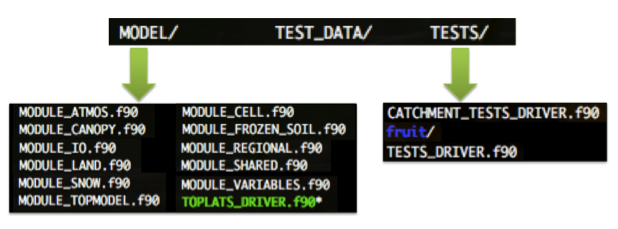
\includegraphics[width=3.0in]{Figures/Modules1.png}
	\caption{New TOPLATS model}
	\label{Modules1}
\end{figure}

\begin{figure}[h]
	\centering
	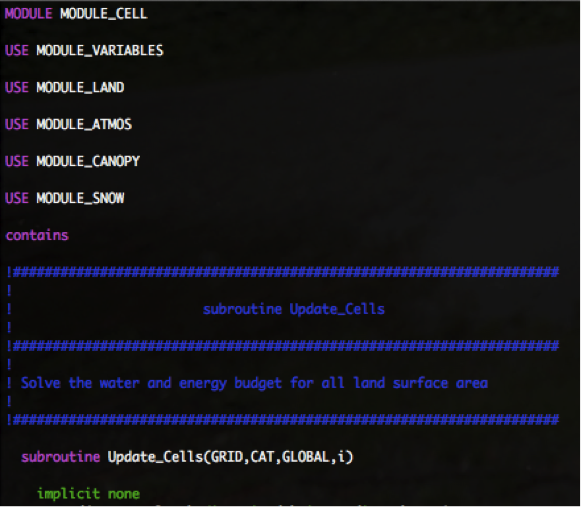
\includegraphics[width=3.0in]{Figures/Modules2.png}
	\caption{Snapshot of MODULE\_CELL.f90}
	\label{Modules2}
\end{figure}

Within each module, as shown in Figure \ref{Modules2}, we first list shared variables and structures from other modules, defined structures being shared by subroutines in the module if there are any, and then list the subroutines that are related to the module. 

\section{Variables}
In the original version of TOPLATS, the variables were stored in one lengthy list. Hundreds of variables were passed into subroutines individually, causing extremely large subroutine calls. For the updated version of TOPLATS developed in this project, these hundreds of variables were organized into derived data types (structures) based upon function or purpose. In this way, structures could be passed into the modules and subroutines in relevant groups, thereby cleaning up the otherwise unmanageable code. In each larger subroutine, such as Atmos, the variables used in the code were replaced with the corresponding member of the structure. For each smaller subroutine, the members of the structures were passed into the subroutine individually to avoid passing in more variables than necessary.

\vspace{1em}

Not only was the original version of TOPLATS crippled by the massive subroutine calls, but it was also impaired by the unreasonable number of help files storing the initialized variables with their corresponding types. Each subroutine was associated with a help file which initialized new variables in each subroutine but which also re-initialized all variables which were passed into the subroutine. This process of re-initializing variables over and over was cumbersome and unnecessary. In the updated version of TOPLATS, the variables in structures are initialized within the structure, and the rest of the variables are only initialized within the larger subroutine in which they are used. In this way, hundreds of files were removed.

\vspace{1em}

Another limitation of the original version of TOPLATS was the use of static memory allocation. Using this method, the size of all arrays needed to be provided at compile time, meaning that the users needed to alter the source files every time they used the model for a different domain. In order to improve upon this, the dynamic memory allocation features implemented in Fortran 90 were used. By dynamically allocating the arrays, the user is able to specify dimensions at run time, allowing for the model to be used across multiple domains without maintaining and compiling multiple versions of the model code.

\section{Tests}

The FORTRAN Unit Test Framework (FRUIT) is used for testing. We have included two test programs: CATCHMENT\_TESTS\_DRIVER and TESTS\_DRIVER, each serving a different purpose.

The CATCHMENT\_TESTS\_DRIVER runs the model and compares all the output variables with the original model over a test catchment. Although written in an inefficient way, the original model's results have been validated, so starting from scratch was unnecessary. To this end, by using the validated output from a sample input data set, all we need to ensure in the catchment tests is that our our modified model reproduces the output at every time step. These tests were contructed first and were run before every commit to ensureno changes to the model predicitons had been made. 

\begin{figure}[h]
	\centering
	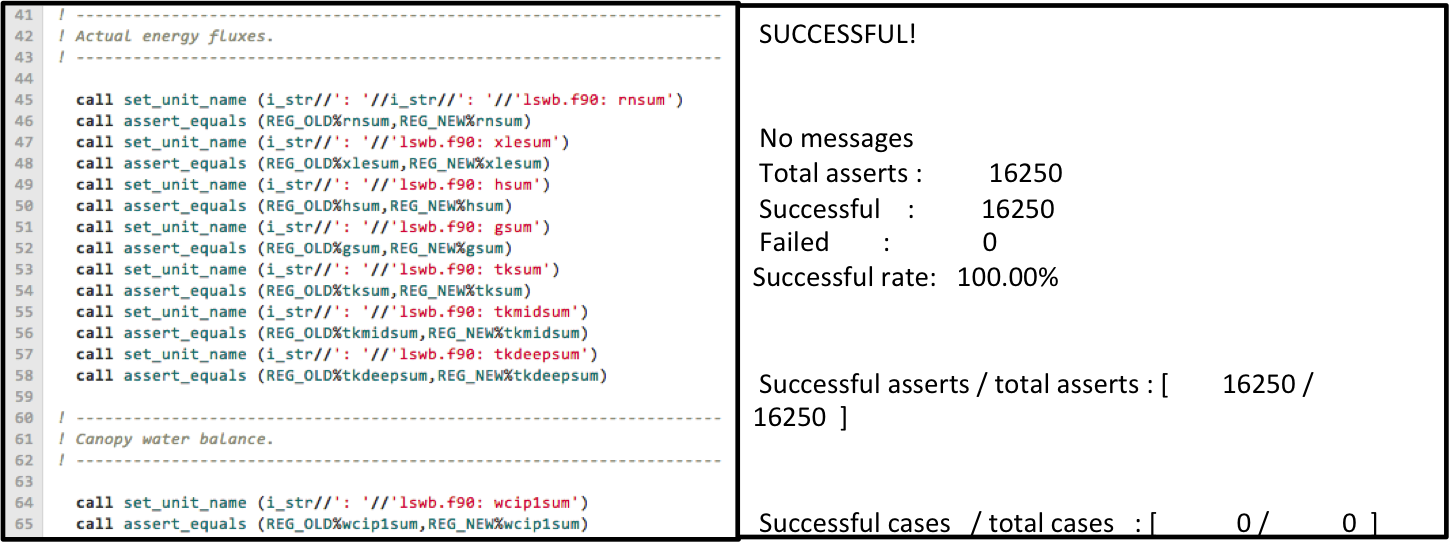
\includegraphics[width=5.5in]{Figures/Tests1.png}
	\label{Tests1}
	\caption{Catchment tests example code (left) and its corresponding assertions output (right)}
\end{figure}

One of the major downfalls of testing the model against old output is the inability to then swap physics. To this end, a set of unit tests were devloped in TESTS\_DRIVER.90 to run tests on the individual subroutines by using random input values.  Considering the amount of subroutines and functions and that the model was previously validated, we only tested about 50 of these subroutines. Random values were given to the subroutine or function being tested, and the resulting value was compared with the true value. The true value was previously calculated by the original subroutine or function. As we move to the next step and we implement new subroutines, we need to ensure that the unit tests capture the same errors as the CATCHMENT\_TESTS.f90 does. This will allow us to eventually replace those tests with the subroutine unit tests.

\begin{figure}[h]
	\centering
	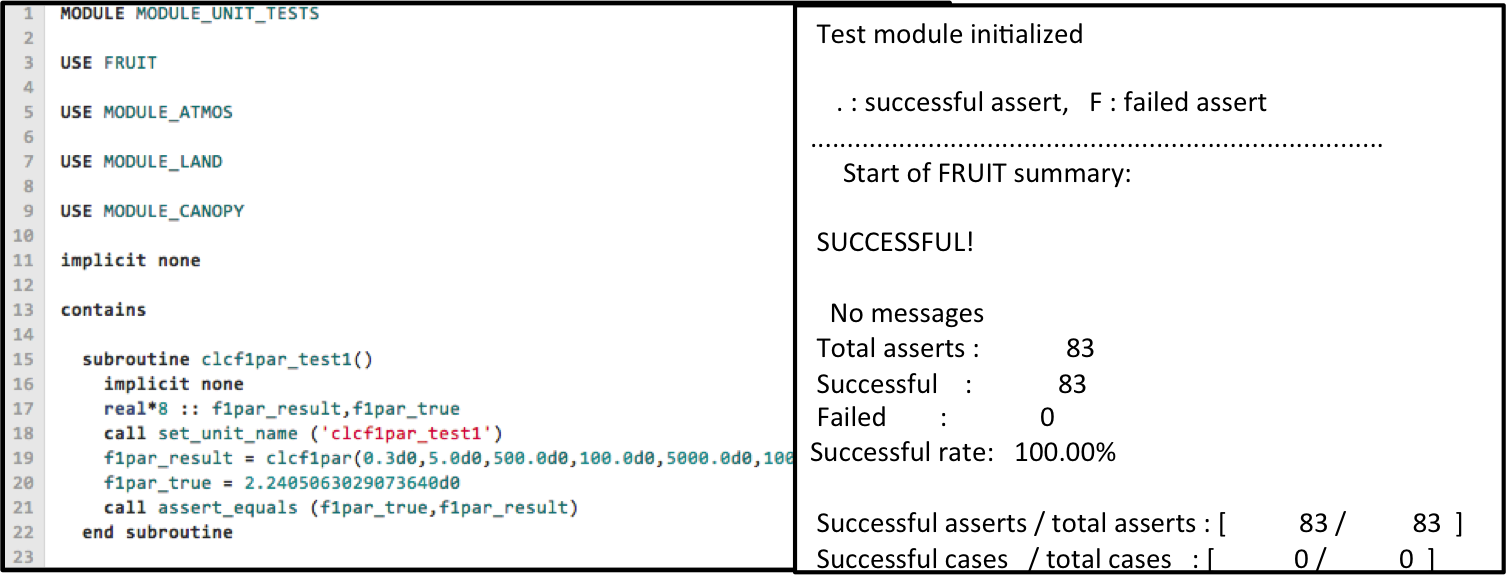
\includegraphics[width=5.5in]{Figures/Tests2.png}
	\caption{Subroutines tests example code (left) and its corresponding assertions output (right)}
	\label{Tests1}
\end{figure}

\section{I/O}

The original model's I/O was extremeley complicated and inefficient. A general file contained a reference to 20+ files that contained the data and parameters. The parameters themselves were split into 10 files, some files having less than 10 parameters. Furthermore, many of the soil and vegetation properties were defined in ascii files which would become unmanageable when the model is taken to global scales. 

For these reasons, a concerted effort was placed on revamping the model's I/O. First, the input file is redefined as the general parameters file. In this file all of the parameters are defined and the user can access the README or manual online to learn about the parameters. The soil and vegetation properties were converted to a flat binary format. The files can be prepared using GrADS, a tool commonly used in meteorology and hydrology. This speeds up the read time, and allows much smaller files. The input forcing data (boundary conditions) are now given through one large layered flat binary file also following the GrADS format. This allows the model to run without having to open/close files every time step. The output data also follows the GrADS format and can be accessed from either GrADS, python, or matlab, among others, given that the user understands how to read flat binary files using these programs. In the near future, we are looking to move towards a netCDF or HDF5 format which is more universal and easier to manage.

\section{Parallelization}

Parallelization is currently implemented using OpenMP. The user can define at runtime how many cores to use. In order to do this, for each time step, the domain is split up into equal sized blocks and then is distributed among the threads. Calculations are then performed for each cell before the domain is reassembled and the regional processes are calculated. For the domain size that we are using the parallelization does not have a significant impact on the calculation time. It should be noted though that for future work, as the domain size increases, we believe that we will find that parallelization becomes increasingly important. In order to run the model on a global scale, we plan to implement parallelization through MPI in order to maximize the computational power of each node.

\section{Variable Initialization}
The current version of TOPLATS was checked for memory leaks and other issues using valgrind. This process identified a number of uninitialized variables which were passed into a subroutine. If the variables were reassigned, this method would not be an issue, but the variables were often used as sums, and if the variables were not initialized to zero, the variables could have any starting value. 

\vspace{1em}

These issues were fixed initially by using the -finit-local-zero option available in gfortran. This option set all uninitialized values to 0 at runtime, which temporarily fixed the problem. However, because we would like to use this model with other compilers, these issues were identified and removed from the code manually using valgrind. After solving these issues, we were successfully able to remove the -finit-local-zero option, and the valgrind analysis found that no memory leaks were occurring in our model.

\section{Profiling}

We used gprof to examine the run time statistics and determine what portions of the code are taking the most time to run. We then used gprof2dot to convert the ascii output into a call graph visualization as shown in Figure \ref{Profiling1}. 

\begin{figure}[h]
	%\centering
	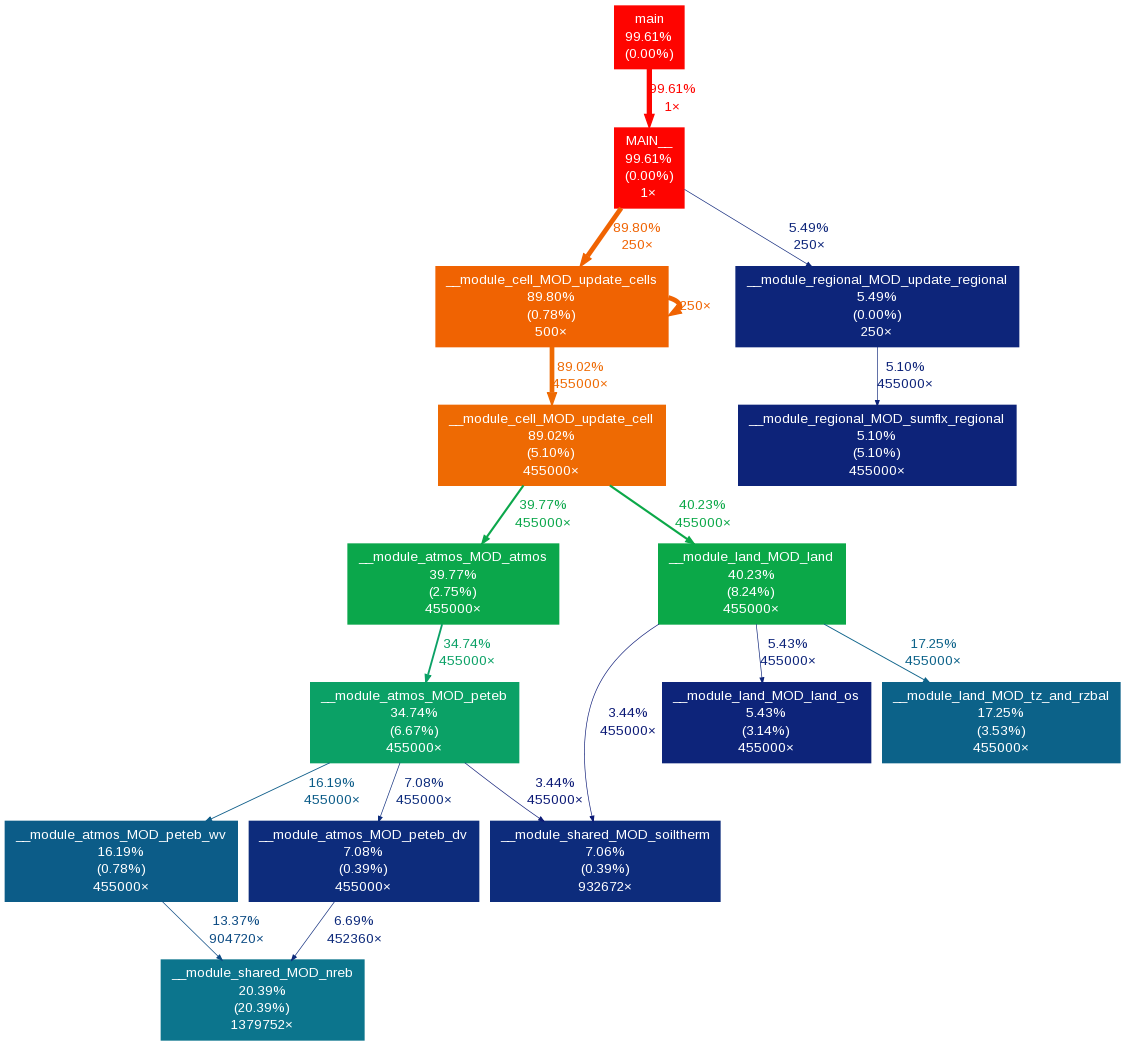
\includegraphics[width=5.0in]{Figures/CallGraph.png}

	\caption{Schematic of the call-graph of TOPLATS. We define a threshold of 5\%, below which all subroutines are discarded from the view. This offers a detailed view on where the model is spending most of its time.}
	\label{Profiling1}
\end{figure}

\vspace{1em}

As expected, the model spends a large amount of its time in the Update\_Cell module (~90\%). This result is mainly caused by the need to ensure energy balance closure. Energy balance closure means that the surface energy balance equation for each grid cell at each time step needs to be minimized. Any future improvement in performance (excluding parallelization) will need to address the nreb subroutine and use more efficient algorithms. Although there is room for improvement, we are happy with the performance of the model. The current runtime for 250 time steps over a 60X66 domain is around 5 seconds. In comparison, this runtime is much faster than most other hydrologic models that thoroughly solve the groundwater interactions between cells.

\newpage
\section{Documentation}

For this project, the documentation was done using a combination of Doxygen and a Readme file for the manual. The Doxygen webpage is organized to show the model flow as well as all subroutines, functions, and variables. Relevant comments have been included for each subroutine using Doxygen syntax so that the user can easily identify the major processes and flow of the model. The Doxygen for this project can be found \href{http://hydrology.princeton.edu/~nchaney/TOPLATS_HTML/index.html}{here}. Additionally, the Readme manual describes hwo to run the model with the given data files and how to provide new data inputs. This Readme is viewable either on Github \href{https://github.com/chaneyn/TOPLATS/wiki/Manual}{here} or as part of the repository.

\section{Conclusion}

As described above, we have accomplished our major goals for this project. The changes to the original model included that derived data types were implemented (although not completely), modules were set up to simplify the code and make it simple to swap physics in the future, the I/O components were separated from other routines and enhanced, parallelization using OpenMP was added, and the main program was replaced with a much cleaner interface. 

\vspace{1em}
These changes will enable us to use this outdated model for future hydrologic studies. Currently, our group is looking at adding the MPI parallelization capability for much larger scale domains. Nathaniel Chaney is currently developing a global model run at a 500 meter spatial resolution on the Blue Waters supercomputer in Illinois. This global model will be groundbreaking work that works to redefine how the global water balance is modeled.

This project and this course have been beneficial to everyone in the project. We have learned how to effectively collaborate on the same program with great help from Github and Git for version control. Testing has become an important part of our programming practices, one which was almost absent before taking this course. Additionaly, learning how to use valgrind has been extremely useful as it also served as an effective debugger for our code. In conclusion, all the tools we have used, github, Doxygen, Valgrind , gprof, etc... will continue to serve as our programming companions in the future.


\end{document}
